\documentclass[15pt,a4paper]{article}

\usepackage[portuguese]{babel}
\usepackage[utf8]{inputenc}
\usepackage{indentfirst}
\usepackage{graphicx}
\usepackage{verbatim}


\begin{document}

\setlength{\textwidth}{16cm}
\setlength{\textheight}{22cm}

\title{\Huge\textbf{Moai}\linebreak\linebreak\linebreak
\Large\textbf{Relatório Intercalar}\linebreak\linebreak

\includegraphics[height=6cm, width=7cm]{feup.pdf}\linebreak \linebreak
\Large{Mestrado Integrado em Engenharia Informática e Computação} \linebreak \linebreak
\Large{Programação em Lógica}\linebreak
}

\author{\textbf{Grupo 5:}\\ Paulo Jorge de Faria dos Reis - 080509037 \\ Miguel Rossi Seabra - 060509054 \\\linebreak\linebreak \\
 \\ Faculdade de Engenharia da Universidade do Porto \\ Rua Roberto Frias, s\/n, 4200-465 Porto, Portugal \linebreak\linebreak\linebreak
\linebreak\linebreak\vspace{1cm}}
%\date{4 de Novembro de 2012}
\maketitle
\thispagestyle{empty}

%************************************************************************************************
%************************************************************************************************

\newpage

\section*{Resumo}
Pretende-se com este relatório apresentar o procedimento seguido pelo grupo de trabalho no desenvolvimento em Prolog do jogo ''Moai''.
\\
Será disponibilizada informação relativamente ao jogo em termos de regras, descrição do tabuleiro, opções tomadas pelo grupo em pontos onde a informação do criador do daquele não é clara e também a apresentação dos predicados de Prolog que foram utilizados para o desenvolvimento do projeto.
\\Também é descrito o possível interface para comunicação com um cliente via sockets.

\newpage

\tableofcontents

%************************************************************************************************
%************************************************************************************************

%*************************************************************************************************
%************************************************************************************************

\newpage

\section{Introdução}
A implementação das regras de um jogo de tabuleiro recente, utilizando programação em lógica apresenta um desafio aliciante, ao mesmo tempo que possibilita o contacto e desenvolvimento de capacidades nesta área aos elementos envolvidos no desenvolvimento deste sistema. É também de ressalvar a criação de um programa funcional que permite a realização de partidas de ''Moai'' onde os intervenientes podem ser humanos ou computadores, e neste caso tendo o sistema capacidades mínimas de realizar jogadas válidas de acordo com as regras. A versão base apenas permitirá a interação em modo de texto através da consolo de Prolog, podendo no entanto ser providenciada a integração com interface gráfico, opção especificada mais adiante.

%*************************************************************************************************
%************************************************************************************************

\section{Descrição do Problema}
O jogo foi criado por Rey Alicea em 2012 \cite{gamegeek}, e não existe qualquer referência histórica deste. Pelo que nos apercebemos o jogo encontra-se ainda num estádio de revisão do mesmo. A descrição das regras \cite{blog, gamegeek} não são claras o suficiente, deixando muito espaço para a interpretação das mesmas, assim a equipa de desenvolvimento das regras em Prolog decidiu utilizar a regras conforme se explica mais adiante.
\\
São necessários dois jogadores para realizar uma partida de ''Moai''.

\section{Arquitetura do Sistema}
O projeto foi desenvolvido num único módulo, pois não se considerou necessário a separação dos predicados de acordo com qual tipo de classificação.
Existem predicados para cada uma das tarefas necessárias à realização de um jogo de \textbf{''Moai''}, os quais são explicados na próxima secção. Bem como a forma como interagem entre si para a obtenção de um resultado útil do programa desenvolvido em Prolog.\\

Por não ser necessário a qualquer um dos autores não foi desenvolvida a componente de comunicação por sockets, a qual mesmo assim foi acautelada pelo facto de cada um dos principais predicados aceitar como variáveis de entrada, entre outras, o estado do jogo, permitindo desta forma a possibilidade de utilizar o programa de uma forma \textit{stateless}, sendo o estado mantido no cliente. Temos assim um paradigma REST que pode também ser utilizado com a interface adequada para a utilização deste projeto em aplicações Web.\\

Para efeitos de demonstração das capacidades do programa existe um predicado (\textit{new\_game}), que inicia um jogo completo de \textbf{''Moai''} utilizando para tal os principais predicados do programa, mas também alguns auxiliares cuja utilidade se fica pela interface com os jogadores e a manutenção de estado do jogo.\\

\subsection{Comunicação por sockets}
Numa eventual implementação da comunicação por sockets seriam consideradas as mensagens conforme se descreve de seguida.\\


\textbf{Início de comunicação}\\
\textit{initialize(X, Y)} $\rightarrow$ \\
\indent\indent\indent\indent	 $\leftarrow$ \textit{ok(Board)}\\
Pedido de inicialização com especificação das dimensões do tabuleiro pretendido, como resposta é devolvida a representação do tabuleiro (lista de listas), representado por \textit{Board}.
Corresponde ao predicado \textit{new\_board(X, Y, Board)}, sendo X e Y as dimensões do tabuleiro, respetivamente em colunas e linhas.
\\


\textbf{Pedido de posicionamento de peão}\\
\textit{ini\_posicao(IBoard, Piece, X, Y)} $\rightarrow$  \\
\indent\indent\indent\indent	$\leftarrow$ \textit{ok(OBoard)}\\
\indent\indent\indent\indent	$\leftarrow$ \textit{invalid}\\
\textit{IBoard} é o estado inicial do tabuleiro, \textit{Piece} pode ser  ''B'' ou ''P'' (corresponde a jogador Branco ou jogador Preto). X e Y são a posição pretendida para colocar o peão. 
A primeira ação do jogo consiste em cada jogador colocar numa casa livre o seu peão. Utilizando o predicado \textit{set\_piece(IBoard, Piece, X, Y, OBoard)} obtemos o tabuleiro (\textit{OBoard}) com a peça do jogador já posicionada se tal for válido, caso contrário a resposta será \textit{invalid}.
\\


\textbf{Pedido de execução de movimento humano}\\
\textit{execute(IBoard,  Push, Player, X, Y)} $\rightarrow$ \\
\indent\indent\indent\indent	$\leftarrow$ \textit{ok(OBoard)}\\
\indent\indent\indent\indent	$\leftarrow$ \textit{invalid}\\
\textit{IBoard} é o estado inicial do tabuleiro, \textit{Push} é a direção de movimento do peão (''s'' para aproximar do bloqueador, ''n'' para afastar), \textit{Player} corresponde ao peão que se pretende mover (''s'' para o Preto, ''n'' para o Branco), X e Y são a posição pretendida para colocar o bloqueador. 
Trata-se de um pedido de movimento de jogador humano, se o movimento não for possível, responder com \textit{invalid} e não realizar qualquer outra operação, se for um movimento válido devolver novo estado do Tabuleiro (\textit{OBoard}).\\
Utiliza o predicado \textit{make\_a\_move(IBoard,  Push, Player, X, Y, OBoard)} para dar a resposta.
\\


\textbf{Pedido de execução de movimento de computador}\\
\textit{calculate(IBoard,  Level, Player)} $\rightarrow$ \\
\indent\indent\indent\indent	$\leftarrow$ \textit{ok(Push, Piece, X, Y, OBoard)}\\
\indent\indent\indent\indent	$\leftarrow$ \textit{invalid}\\
\textit{IBoard} é o estado inicial do tabuleiro,  \textit{Level} o nível de dificuldade pretendido e  \textit{Player} qual o jogador que está a realizar a jogada (''s'' para o Preto, ''n'' para o Branco).
Utiliza-se para solicitar um movimento a realizar pela AI a favor de um jogador (Player), em resposta utiliza-se o resultado do predicado \textit{create\_a\_move(IBoard, Level, Player, Push, Piece, X, Y, OBoard)} onde \textit{Push} é a direção que o peão foi movido (''s'' foi aproximado do bloqueador, ''n'' foi afastado), \textit{Piece} qual o peão que foi movido (''s'' para o Preto, ''n'' para o Branco), X e Y são a posição onde o bloqueador foi colocado e o novo estado do Tabuleiro é (\textit{OBoard}).
Se não for possível realizar um movimento devolver  \textit{invalid}, nesta situação o cliente deveria fazer uma verificação de final de jogo.\\


\textbf{Verificação de final de jogo}\\
\indent\indent\indent\indent	$\leftarrow$ \textit{game\_end(Board, Piece)}\\
\indent\indent\indent\indent	$\leftarrow$ \textit{ok(Player}\\
Atendendo à forma de definir o vencedor neste jogo, apenas o estado do tabuleiro  (\textit{Board}) não basta para se definir o vencedor. Ambos os peões podem estar a certo momento bloqueados, o jogador que estiver a iniciar a jogada é que será o derrotado porque pelas regras a sua peça tem de ter a possibilidade de se mover no inicio da sua jogada. Por isso tem também de dizer qual o jogador a testar o final de jogo utilizando ''P'' ou ''B'' em \textit{Piece}. A resposta obtida do predicado \textit{endgame(Board, Piece)} será \textbf{true} se o jogador perdeu ou \textbf{false} se ganhou.\\


\textbf{Fim da comunicaçao}\\
\indent\indent\indent\indent	$\leftarrow$ \textit{bye}\\
\indent\indent\indent\indent	$\leftarrow$ \textit{ok}\\
Informa da vontade de terminar a comunicação, permitindo a libertação de recursos.\\


\section{Módulo de Lógica do Jogo}
Para realizar um jogo inicia-se com o predicado \textit{new\_game}, o qual apresenta as regras do jogo (\textit{print\_help}) e coloca uma série de questões ao utilizador (\textit{setup\_game}, as quais permitem inicializar o mesmo. O controlo é então passado para \textit{main\_loop}.\\


O \textit{main\_loop} recebe o estado do tabuleiro e o actual jogador. O primeiro jogador é o preto ''P'' (alternando com o branco ''B'') e o tabuleiro que foi criado em \textit{setup\_game}. A primeira operação é verificar se o jogo terminou com a vitória do jogador anterior, usando \textit{endgame}. De seguida é questionada a posição pretendida para o bloqueador (Coluna e Linha), a ação pretendida (puxar ou empurrar) e o peão sobre o qual se pretende aplicar (preto ou branco). Com esta informação chama-se o predicado \textit{make\_a\_move} que irá processar as operações pretendidas. É apresentado na consola o novo tabuleiro (\textit{print\_board}) e definido o próximo jogador (\textit{next\_piece}). Faz-se então uma chamada recursiva ao \textit{main\_loop}.\\

O \textit{make\_a\_move} vai fazer o parse dos argumentos e consoante o tipo de movimento especificado vai chamar o predicado respetivo para esse movimento. Este último irá utilizar os predicados de pesquisa, clarificados abaixo na ''Validação de Jogadas'', por forma a tentar encontrar o peão pretendido em linha com o bloqueador colocado pelo jogador nessa mesma jogada. No caso de se encontrar o peão numa das pesquisas o movimento é então realizado com a respetiva atualização do tabuleiro, caso contrário \textbf{false} é retornado.\\


Em caso de jogada válida o tabuleiro é atualizado com a colocação de um bloqueador na posição pedida pelo jogador e com a deslocação do peão solicitado da posição antiga, que fica vazia, para a sua nova posição.\\


\subsection{Visualização do Estado do Jogo}
\textit{print\_board(+Board).}\\
Recebe uma representação do estado do tabuleiro e imprime-o na consola, conforme figura 1.\\
\textit{Board} Representação do estado do tabuleiro, na forma de uma lista de listas (lista de linhas do tabuleiro).\\
\begin{figure}[h!]
\begin{center}
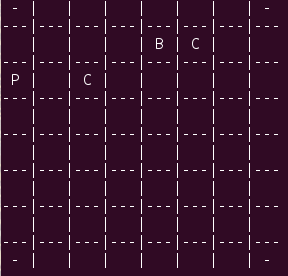
\includegraphics[height=5cm,width=5cm]{tabuleiro_meio.png}
\caption{Tabuleiro durante o jogo}
\label{fig:tabuleiro_meio}
\end{center}
\end{figure}


\subsection{Validação de Jogadas} 
\textit{search\_horizontal\_forward(+IBoard, +Piece, +XCounter, +YCounter, -PieceX, -PieceY).}\\
\textit{search\_vertical\_forward(+IBoard, +Piece, +XCounter, +YCounter, -PieceX, -PieceY).}\\
\textit{search\_diagonal\_forward(+IBoard, +Piece, +XCounter, +YCounter, -PieceX, -PieceY).}\\
\textit{search\_reverse\_diagonal\_forward(+IBoard, +Piece, +XCounter, +YCounter, -PieceX, -PieceY).}\\
\textit{search\_horizontal\_backward(+IBoard, +Piece, +XCounter, +YCounter, -PieceX, -PieceY).}\\
\textit{search\_vertical\_backward(+IBoard, +Piece, +XCounter, +YCounter, -PieceX, -PieceY).}\\
\textit{search\_diagonal\_backward(+IBoard, +Piece, +XCounter, +YCounter, -PieceX, -PieceY).}\\
\textit{search\_reverse\_diagonal\_backward(+IBoard, +Piece, +XCounter, +YCounter, -PieceX, -PieceY).}\\
Este conjunto de predicados permite validar verificar se o peão (\textit{Piece}) se encontra na linha que está a ser testada, numa posição que permite o movimento para ou a afastar-se deste.\\
\textit{IBoard} é a representação inicial do tabuleiro.\\
\textit{Piece} O peão para o qual se pretende fazer a validação (''P'' ou ''B'').\\
\textit{XCounter} Coluna onde se pretende colocar o bloqueador (inteiro).\\
\textit{YCounter} Linha onde se pretende colocar o bloqueador (inteiro).\\
\textit{PieceX} Coluna onde se encontra o peão (caso o movimento possa ser realizado, \textbf{false} em caso contrário).\\
\textit{PieceY} Linha  onde se encontra o peão (caso o movimento possa ser realizado, \textbf{false} em caso contrário).\\
\begin{figure}[h!]
\begin{center}
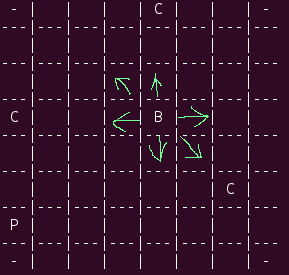
\includegraphics[height=5cm,width=5cm]{tabuleiro_movimento.png}
\caption{Tabuleiro com Movimentos possíveis}
\label{fig:tabuleiro_movimento}
\end{center}
\end{figure}


\subsection{Execução de Jogadas}
\textit{move(+IBoard, +XCounter, +YCounter, +Piece, +PushPull, -OBoard).}\\
Cada jogador na sua vez tem de fazer duas ações que por estarem relacionadas são tratadas num único predicado, indicando o estado inicial do tabuleiro e a descrição da jogada a realizar, caso seja válida temos de volta o novo estado do tabuleiro, ou \textbf{false} caso contrário.\\
\textit{IBoard} é a representação inicial do tabuleiro.\\
\textit{XCounter} Coluna onde se pretende colocar o bloqueador (inteiro).\\
\textit{YCounter} Linha onde se pretende colocar o bloqueador (inteiro).\\
\textit{Piece} O peão para o qual se pretende fazer a validação (''P'' ou ''B'').\\
\textit{PushPull} Direção do movimento pretendida (''push'' ou ''pull'').\\
\textit{OBoard} é a representação final do tabuleiro.\\


\subsection{Final do Jogo}
\textit{endgame(+Board, +Piece).}\\
Devido ás regras do jogo, apenas pelo estado do tabuleiro não é possível determinar um vencedor, também temos de saber qual o jogador que vai iniciar a sua ação. Como resposta temos \textbf{false} ou \textbf{true} conforme o jogador ganhou ou perdeu.\\
\textit{IBoard} é a representação inicial do tabuleiro.\\
\textit{Piece} O peão para o qual se pretende fazer a validação (''P'' ou ''B'').\\

\subsection{Rotina de jogo}
\textit{main\_loop(+Board, +Piece}\\
Para que se possa jogar ''Moai'' utilizando apenas o interpretador de Prolog, temos este predicado que controla a interface com o utilizador e mantêm o estado do jogo durante a sua execução.\\
\textit{IBoard} é a representação inicial do tabuleiro.\\
\textit{Piece} O peão para o qual se pretende fazer a validação (''P'' ou ''B'').\\


Não foram descritos os predicados auxiliares por não se considerar de utilidade e porque iriam aumentar consideravelmente a dimensão deste relatório sem ganho significativo.\\


\section{Interface com o Utilizador}
Não foi implementado o módulo de comunicação com o visualizador. A Interface com o utilizador é feita através de predicados do próprio Prolog.\\
\begin{figure}[h!]
\begin{center}
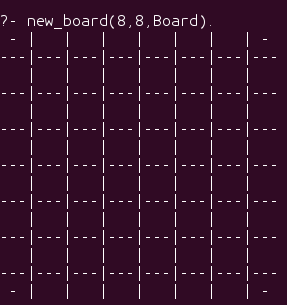
\includegraphics[height=5cm,width=5cm]{tabuleiro_vazio.png}
\caption{Tabuleiro vazio}
\label{fig:tabuleiro_vazio}
\end{center}
\end{figure}
Para iniciar um novo jogo deve-se utilizador o predicado \textit{new\_game}, de seguida devemos informar as dimensões do tabuleiro que pretendemos utilizar, para tal devem ser introduzido um valor inteiro seguido de . (ponto) para cada uma das dimensões.
Uma vez que cada jogador pode ser controlado por um humano ou pela AI do computador, temos de responder cada um dos jogadores é humano ou não usando \textit{s} ou \textit{n}.\\
A primeira ação de cada um dos jogadores, Branco e depois o Preto (representados no tabuleiro por ''B'' e ''P'' respetivamente), é a colocação do seu peão no tabuleiro, para tal é perguntado ao utilizador qual a Coluna  (X) e a Linha (Y) onde ele o pretende colocar, se for uma posição válida o tabuleiro é atualizado. A partir deste ponto, começando pelo Jogador Branco e alternando com o Jogador Preto, até que se alcance a condição de vitória (derrota) de um deles terminando assim o jogo, realizam-se jogadas de acordo com as regras já enunciadas neste relatório.\\
Na sua vez, cada jogador informa a Coluna (X) e a Linha (Y) onde pretende colocar o bloqueador (representado por ''C'' no tabuleiro), se pretende empurrar (''s'') ou puxar (''n'') o peão em relação ao bloqueador, e também qual o peão sobre o qual pretende atuar, ''s'' para Preto e ''n'' para Branco.

\emph{Nota:} A razão para utilizar ''n'' e ''s'' em algumas das respostas quando a resposta adequada deveria ser outra (''P'' ou ''B'' por exemplo) está relacionada com o reaproveitamento em várias situações distintas de código que foi adaptado de predicados obtidos na Internet \cite{developerzen}.


\section{Conclusões e Perspetivas de Desenvolvimento}
Utilizar o Prolog para definir as regras de um jogo é algo relativamente simples, sendo apenas necessário a definição de um conjunto de predicados (regras) que descrevam o que é ou não possível fazer no jogo. A comunicação com o utilizador é bem complicada de desenvolver neste contexto, sendo responsável por grande parte do tempo utilizado no desenvolvimento do programa.


A definição de regras passa pela elaboração de factos que definem condições de paragem e clausulas com predicados que permitem o processamento de casos gerais.


Apenas foi desenvolvido o suficiente para possibilitar o jogo entre 2 humanos, a componente de inteligência artificial necessária para que um ou os dois jogadores sejam controlados pelo computador não foi desenvolvida, este é sem dúvida a principal falha e onde reside a possibilidade de melhoria do programa.


A comunicação via sockets passaria também pela criação de um predicado (mais auxiliares) que fizessem a interpretação das mensagens dos clientes e enviassem a resposta a estes, pois a definição da interface está feita, assim como os principais predicados necessários.


\clearpage
\addcontentsline{toc}{section}{Bibliografia}
\renewcommand\refname{Bibliografia}
\bibliographystyle{plain}
\bibliography{myrefs}

\listoffigures

\newpage
\appendix
\section{Nome do Anexo A}
\begin{verbatim}
Código Prolog implementado devidamente comentado e outros elementos úteis que não sejam essenciais ao relatório.


\end{verbatim}
\end{document}
